\def\ArtDir{main/}%% Trim Size: 9.75in x 6.5in
%% Text Area: 8in (include Runningheads) x 5in
%% ws-ijprai.cls   :   8-8-2014
%% Class file to use with ws-ijprai.tex written in Latex2E.
%% The content, structure, format and layout of this style file is the
%% property of World Scientific Publishing Co. Pte. Ltd.
%% Copyright 2014 by World Scientific Publishing Co.
%% All rights are reserved.
%%%%%%%%%%%%%%%%%%%%%%%%%%%%%%%%%%%%%%%%%%%%%%%%%%%%%%%%%%%%%%%%%%%%%%%%%%%%
%

\documentclass{ws-ijprai}
\def\ArtDir{main/}
\begin{document}

\markboth{Authors' Names}{Instructions for Typing Manuscripts (Paper's Title)}

%%%%%%%%%%%%%%%%%%%%% Publisher's area please ignore %%%%%%%%%%%%%%%
%
\catchline{}{}{}{}{}
%
%%%%%%%%%%%%%%%%%%%%%%%%%%%%%%%%%%%%%%%%%%%%%%%%%%%%%%%%%%%%%%%%%%%%
\title{Template for International Journal of Pattern Recognition and Artificial Intelligence - IJPRAI}
%\title{Instructions for Typesetting Camera-Ready \\
%Manuscripts using \TeX\ or \LaTeX\footnote{For the title, try not to use
%more than 3 lines. Typeset the title in 10 pt Roman, boldface with the first letter of important words capitalized.}}

\author{First Author\footnote{Typeset names in 8~pt Roman.
Use the footnote to indicate the present or permanent
address of the author.}}

\address{University Department, University Name, Address\\
City, State ZIP/Zone,Country\,\footnote{State without abbreviations,
the affiliation and mailing address, including country.
Typeset in 8~pt italic.}\\
\email{author\_id@domain\_name\footnote{Typeset author e-mail address in single line}}
\http{$<$webaddress$>$}}

\author{Second Author}

\address{Group, Laboratory, Address\\
City, State ZIP/Zone, Country\\
author\_id@domain\_name}

\maketitle

%begin{history}
%received{(Day Month Year)}
%revised{(Day Month Year)}
%accepted{(Day Month Year)}
%comby{(xxxxxxxxxx)}
%end{history}

\begin{abstract}
The abstract should summarize the context, content
and conclusions of the paper in less than 200 words. It should
not contain any reference citations or displayed equations. Typeset the
abstract in 8~pt roman with baselineskip of 10~pt, making
an indentation of 1.5 pica on the left and right margins.
\end{abstract}

\keywords{Keyword1; keyword2; keyword3.}

\section{General Appearance}

Contributions to the {\it International Journal of Pattern Recognition
and Artificial Intelligence} will mostly be processed
by using the authors' source files. These should be submitted
with the manuscripts, and resubmitted in the final form if a paper
requires revision before being accepted for publication.

\section{The Main Text}

Authors are encouraged to have their contribution checked for grammar.
American spelling should be used. Abbreviations are allowed but should
be spelt out in full when first used. Integers ten and below are to be
spelt out. Italicize foreign language phrases (e.g.~Latin, French).

The text is to be typeset in 10~pt roman, single spaced with
baselineskip of 13~pt. Text area (including copyright block) is
8 inches high and 5 inches wide for the first page. Text area
(excluding running title) is 7.7 inches high and 5 inches wide for
subsequent pages. Final pagination and insertion of running titles
will be done by the publisher.

\section{Major Headings}

Major headings should be typeset in boldface with the first letter of
important words capitalized.

\subsection{Sub-headings}

Sub-headings should be typeset in boldface italic and capitalize
the first letter of the first word only. Section number to be in
boldface roman.

\subsubsection{Sub-subheadings}

Typeset sub-subheadings in medium face italic and capitalize the
first letter of the first word only. Section numbers to be in
roman.

\subsection{Numbering and spacing}

Sections, sub-sections and sub-subsections are numbered in
Arabic.  Use double spacing before all section headings, and
single spacing after section headings. Flush left all paragraphs
that follow after section headings.

\subsection{Lists of items}

List may be presented with each item marked by bullets and numbers.

\subsection*{Bulleted items}

\begin{itemlist}
 \item item one,
 \item item two,
 \item item three.
\end{itemlist}

\subsection*{Numbered items}

\begin{arabiclist}
 \item item one,
 \item item two,
 \item item three,
\end{arabiclist}

The order of subdivisions of items in bullet and numbered lists may be
presented as follows:

\subsection*{Bulleted items}

\begin{itemize}
\item First item in the first level
\item Second item in the first level
\begin{itemize}
\item First item in the second level
\item Second item in the second level
\begin{itemize}
\item First item in the third level
\item Second item in the third level
\end{itemize}
\item Third item in the second level
\item Fourth item in the second level
\end{itemize}
\item Third item in the first level
\item Fourth item in the first level
\end{itemize}

\subsection*{Numbered items}

\begin{arabiclist}
\item First item in the first level
\item Second item in the first level
\begin{alphlist}[(a)]
\item First item in the second level
\item Second item in the second level
\begin{romanlist}[iii.]
\item First item in the third level
\item Second item in the third level
\item Third item in the third level
\end{romanlist}
\item Third item in the second level
\item Fourth item in the second level
\end{alphlist}
\item Third item in the first level
\item Fourth item in the first level
\end{arabiclist}

\section{Equations}

Displayed equations should be numbered consecutively, with the number
set flush right and enclosed in parentheses. The equation numbers
should be consecutive within the contribution.

\begin{equation}
\mu(n, t) = \frac{\sum^\infty_{i=1} 1(d_i < t, N(d_i)
= n)}{\int^t_{\sigma=0} 1(N(\sigma) = n)d\sigma}\,.
\label{eq:jaa}
\end{equation}

Equations should be referred to in abbreviated form,
e.g.~``Eq.~(\ref{eq:jaa})'' or ``(2)''. In multiple-line equations,
the number should be given on the last line.

Displayed equations are to be centered on the page width.  Standard
English letters like x are to appear as $x$ (italicized) in the text
if they are used as mathematical symbols. Punctuation marks are used
at the end of equations as if they appeared directly in the text.

\section{Theorem environments}

\begin{theorem}\label{thm1}
Theorems, lemmas, definitions, etc. are set on a separate paragraph,
with extra 1 line space above and below. They are to be numbered
consecutively within the contribution.
\end{theorem}

\begin{lemma}[Optional Heading]\label{lem1}
Theorems, lemmas, definitions, etc. are set on a separate paragraph,
with extra 1 line space above and below. They are to be numbered
consecutively within the contribution.
\end{lemma}

\begin{proof}
Proofs should end with
\end{proof}

\section{Illustrations and Photographs}

Figures are to be inserted in the text nearest their first reference.
Figure placements can be either top or bottom.  Original india ink
drawings of glossy prints are preferred. Please send one set of
originals with copies. If the author requires the publisher to reduce
the figures, ensure that the figures (including letterings and
numbers) are large enough to be clearly seen after reduction. If
photographs are to be used, only black and white ones are acceptable.

\begin{figure}[bh]
\centerline{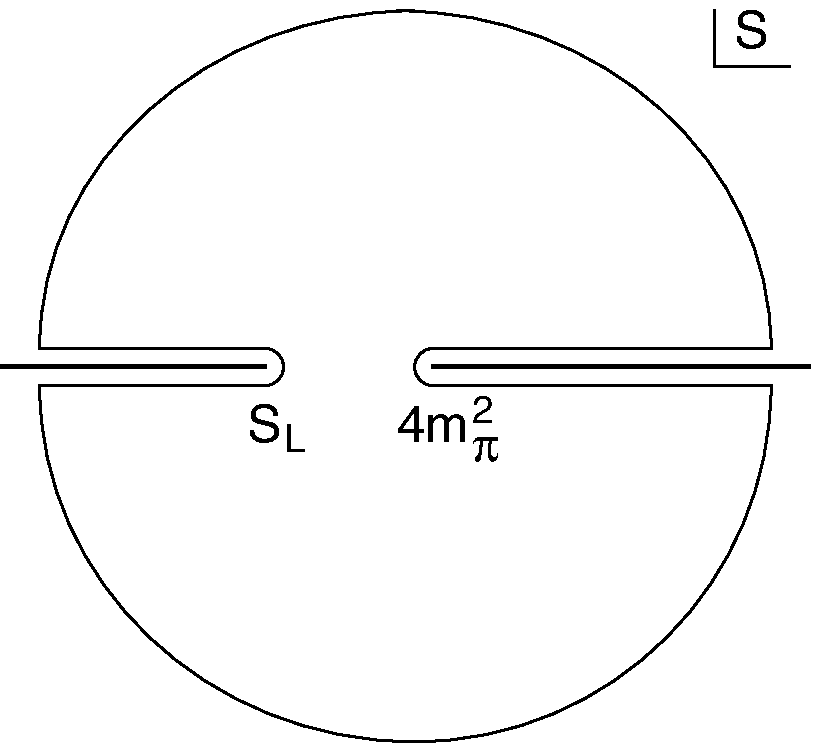
\includegraphics[width=5cm]{ijpraif1}}
\vspace*{8pt}
\caption{A schematic illustration of dissociative recombination. The
direct mechanism, 4m$^2_\pi$ is initiated when the
molecular ion S$_{\rm L}$ captures an electron with kinetic energy.}
\end{figure}

Figures are to be sequentially numbered in Arabic numerals. The
caption must be placed below the figure. Typeset in 8~pt roman with
baselineskip of 10~pt. Long captions are to be justified by the
``page-width''.  Use double spacing between a caption and the text
that follows immediately.

Previously published material must be accompanied by written
permission from the author and publisher.

\section{Tables}

Tables should be inserted in the text as close to the point of
reference as possible. Some space should be left above and below the
table.

Tables should be numbered sequentially in the text in Arabic
numerals. Captions are to be centralized above the tables.  Typeset
tables and captions in 8~pt roman with baselineskip of 10~pt. Long
captions are to be justified by the ``table-width''.

\begin{table}[th]
\tbl{Comparison of acoustic for frequencies for piston-cylinder problem.}
{\begin{tabular}{@{}cccc@{}} \toprule
Piston Mass & Analytical Frequency & TRIA6-$S_1$ Model & \% Error \\
                                             & (Rad/s) & (Rad/s) \\ \colrule
1.0\hphantom{00} & \hphantom{0}281.0 & \hphantom{0}280.81 & 0.07 \\
0.1\hphantom{00} & \hphantom{0}876.0 & \hphantom{0}875.74 & 0.03 \\
0.01\hphantom{0} & 2441.0 & 2441.0\hphantom{0} & 0.0\hphantom{0} \\
0.001 & 4130.0 & 4129.3\hphantom{0} & 0.16\\ \botrule
\end{tabular}}
\begin{tabnote}
Table notes
\end{tabnote}
\begin{tabfootnote}
\tabmark{a} Table footnote A\\
\tabmark{b} Table footnote B
\end{tabfootnote}
\end{table}

If tables need to be extended over to a second page, the continuation
of the table should be preceded by a caption, e.g.~``{\it Table 2.}
$(${\it Continued}$)$''. Notes to tables are placed below the final
row of the table and should be flushleft.  Footnotes in tables should
be indicated by superscript lowercase letters and placed beneath the
table.

\section{Running Heads}

Please provide a shortened runninghead (not more than eight words) for
the title of your paper. This will appear on the top right-hand side
of your paper.

\section{Footnotes}

Footnotes should be labeled sequentially in superscript lowercase
roman letters.\footnote{Footnotes should be typeset in 8~pt roman at
the bottom of the page.}

\section*{Acknowledgments}

This section should come before the References. Funding
information may also be included here.

\appendix

\section{Appendices}

Appendices should be used only when absolutely necessary. If there is
more than\break

\pagebreak

\noindent
one appendix, number them alphabetically. Number displayed
equations occurring in the Appendix in this way, e.g.~(\ref{appeqn}),
(A.2), etc.
\begin{equation}
\mu(n, t) = \frac{\sum^\infty_{i=1} 1(d_i < t, N(d_i)
= n)}{\int^t_{\sigma=0} 1(N(\sigma) = n)d\sigma}\,.
\label{appeqn}
\end{equation}

\section*{References}

References are to be listed alphabetically with Arabic numerals.  They
can be typed in superscripts after punctuation marks, e.g.~``$\ldots$
in the statement.\cite{joliat}'' or used directly, e.g.~``see
Ref.~\refcite{clark} for examples.'' Please list using the style shown
in the following examples.  For journal names, use the standard
abbreviations. Typeset references in 9~pt roman.

\begin{thebibliography}{0}
%1.
\bibitem{beeson} M. J. Beeson, {\it Foundations of Constructive
Mathematics}, Springer, Berlin, 1985.

%2
\bibitem{clark} K. L. Clark, ``Negations as failure,''
{\it Logic and Data Bases}, eds.~H. Gallaire and\break
J. Winker, Plenum Press, NY, 1973, pp.~293--306.

%3
\bibitem{dolve} D. Dolve, ``Unanimity in an unknown and unreliable
environment,'' {\it Proc. 22nd Ann. Symp. Foundations of
Computer Science}, Nashville, TN, Oct. 1981, pp.~159--168.

%4
\bibitem{gewirtz} W. L. Gewirtz, ``Investigations in the theory of
descriptive complexity,'' Ph.~D. Thesis, New York University, 1974.

%5
\bibitem{joliat} M. Joliat, ``A simple technique for partial elimination of
unit productions from LR({\it k}) parsers,'' {\it IEEE Trans. Comput.} {\bf 27} (1976) 753--764.

%6
\bibitem{tamassia} R. Tamassia, C. Batini and M. Talamo,
``An algorithm for automatic layout of entity relationship diagrams,''
{\it Entity-Relationship Approach to Software Engineering,
Proc. 3rd Int. Conf. Entity-Relationship Approach}, eds.~C. G. Davis,
S. Jajodia, P. A. Ng and R. T. Yeh, North-Holland, Amsterdam, 1983,
pp.~421--439.

\end{thebibliography}

\vspace*{-0.01in}
%\vspace*{-0.3in}
\noindent
\rule{12.6cm}{.1mm}

\section*{Biographical Sketch and Photo}

Upon acceptance of an article, a brief biographical sketch and
photograph of each author are to be supplied to the Publisher.

\biophoto{wang}{{\bf Chuan-Cheng Wang} received the
B.S.~degree\break
in electrical engineering from National Sun Yat-Sen University,
Kaoh-\break siung, Taiwan in 1992 and the M.S. degree in
computer science from National Chiao Tung University, Hsinchu,\break
Taiwan in 2001.}

\vglue-1.75truein
\hspace*{2.45truein}
\biophoto{gao}{{\bf Yongsheng Gao} received the B.Sc. and\break
M.Sc. degrees in electronic engineering from\break Zhejiang
University,\break China, in 1985 and 1988 respectively, and the
Ph.D. in computer engineering from Nanyang Technological University,
Singapore. Currently, he is an assistant professor with Nanyang
Technological University, Singapore.}

\end{document}